%!TEX TS-program = xelatex
% see https://www.writelatex.com/coursera/latex/5.2.2

\documentclass[a4paper,12pt]{extarticle}

% Russian fonts
\usepackage[english,russian]{babel}
\usepackage[utf8]{inputenc}
\usepackage{fontspec}
\defaultfontfeatures{Ligatures={TeX},Renderer=Basic}
\setmainfont[Ligatures={TeX,Historic}]{Times New Roman}
\setmonofont{Courier New}
\usepackage{indentfirst}
\usepackage{parskip}
\usepackage{tikz}
\usepackage{hyperref}
\usepackage[nameinlink]{cleveref}
\usepackage{booktabs}
\usepackage{tabularx}
\usepackage{amssymb}
\usepackage{wrapfig}
\usepackage[bottom]{footmisc}
\linespread{1.2}
\hypersetup{final=true}
\addto\captionsngerman{
	% Second argument is singular, third is plural
	\crefname{figure}{abb.}{abb.}
	\Crefname{figure}{Abb.}{Abb.}
}
\crefname{figure}{рис.}{рис.}
\frenchspacing

% Margins
% \usepackage[top=20mm, bottom=20mm, left=25mm, right=10mm]{geometry} % GOST
\usepackage[top=20mm, bottom=20mm, left=20mm, right=20mm]{geometry}

% Paragraph spacing
\setlength{\parindent}{2em}
\setlength{\parskip}{1.2em}
\usepackage{setspace}
\usepackage{graphicx}
\usepackage{tabulary}

\begin{document} % конец преамбулы, начало документа
	{
		\begin{titlepage}
			\setstretch{1}
			\centering
			\textbf{\uppercase{ЮГО-ЗАПАДНОЕ ОКРУЖНОЕ УПРАВЛЕНИЕ ОБРАЗОВАНИЯ\\ДЕПАРТАМЕНТА ОБРАЗОВАНИЯ\\ГОРОДА МОСКВЫ\\\vspace{0.5cm}ГБОУ ШКОЛА №1533 "ЛИТ"}}\par
			\rule{\textwidth}{1pt}\par
			\vspace{2.25cm}
			\large\textbf{ТЕЗИСЫ РАБОТЫ}\par
			\vspace{0.5cm}
			\large(специальность "Прикладное программрование")\par
			\vspace{0.5cm}
			\large{учащегося группы 11.3\\Захарова Ильи Александровича}\par
			\vspace{2cm}
			{\Huge{\textbf{Разработка гипервизора Jinet}}}\par
			\vspace{3cm}
			\begin{flushright}
				\begin{tabular}{rl}
					Научный руководитель:& Байков Б. К.,\\
					& ведущий системный разработчик,\\
					& \flqq Т-Платформы\frqq\\
					& \\
					Консультанты:& Потёмкин А.В\\
					& Гиглавый А.В.\\
					& Завриев Н.К.\\
					& Труфанов Д.С.
					
				\end{tabular}
			\end{flushright}
			\par
			\vfill
			Москва --- 2017
		\end{titlepage}
	}
	\linespread{1.2}
	\tableofcontents
	\linespread{1.2}
	\pagebreak
	\section{Введение}
	
	Гипервизор -- это программа, обеспечивающая разделение ресурсов компьютера на несколько виртуальных машин, и запуск на каждой виртуальной машине своей операционной системы. \par
	Такая программа обеспечивает либо разделяемый, либо монопольный доступ виртуальных машин к каждому из аппаратных устройств компьютера. Создаются виртуальные устройства, конфигурация которых может отличаться от конфигурации устройств аппаратных.\par
	Виртуализация позволяет эффективно и безопасно разделять работающие приложения друг от друга. Виртуальные машины не могут влиять на ход работы друг друга, и, если скомпрометирована одна виртуальная машина, все остальные остаются в безопасности. Поэтому она используется в самых разных областях IT. Зачастую виртуализацию также используют для эффективного сегментирования ресурсов компьютера на отдельные виртуальные машины.\par
	Была поставлена задача написать минимальный учебный демонстрационный гипервизор. Исходный текст проекта выпущен под лицензией MIT.
	\section{Актуальность}
	С каждым годом технологии виртуализации всё глубже и глубже входят в мир информационных технологий, находя применения в самых разных областях IT:
	\begin{enumerate}
		\item изоляция серверных систем для обеспечения их безопасности
		\item эффективное сегментирование ресурсов компьютера
		\item одновременное использование разных ОС на настольном компьютере
		\item отладка гостевых систем через вывод всех выходов из ВМ
	\end{enumerate}
	\par Для создания систем виртуализации требуются специалисты, способные понимать принципы и механизмы программной и аппаратной виртуализации. Для меня, как автора диплома, целью написания диплома стало погружение в мир виртуализации, вычислений и прямого программирования железа. Удалось узнать, как работает виртуализация изнутри и научиться писать код управления механизмами обслуживания виртуализации. \par
	\section{Постановка задачи}
	Идея проекта была предложена руководителем с целью изучения архитектуры x86, включая механизмы изоляции приложений и виртуальных машин друг от друга путём создания монитора виртуальных машин, он же гипервизор. Для меня это стало уникальной возможностью углубить знания архитектуры процессоров Intel и навыки системного программирования. \par
	\textbf{Цель работы} -- это создание минимального монитора виртуальных машин (гипервизора) с использованием механизмов аппаратной виртуализации архитектуры x86-64 (AMD64). \par
	Были поставлены следующие задачи:
	\begin{enumerate}
		\item Обеспечить загрузку из бутсектора (bootsector)
		\item Настроить режим работы видеоадаптера для отображения вывода текстовых данных
		\item Настроить память в 32-битной плоской модели и осуществить переход в 32-битный защищённый режим (\texttt{Protected Mode})
		\item Настроить механизмы страничной трансляции памяти и переход в 64-битный режим (\texttt{Long Mode})
		\item Настроить обработку исключений и прерываний
		\item Настроить расширения аппаратной виртуализации Intel VT-i и включение режима VMX
		\item Обеспечить функционирования вызовов (VMCall) из виртуальных машин в гипервизор (монитор виртуальных машин) и возвратов обратно в виртуальные машины
	\end{enumerate}
	\section{Анализ предметной области}
	\subsection{Виртуализация}
	Виртуализация – техника предоставления исполняемой программе набора вычислительных ресурсов, абстрагированная от их аппаратной реализации. Виртуализация была предметом изучения информатики на протяжении многих лет: так, например, советские инженеры решали проблему портирования программного обеспечения с платформ имеющих другие интерфейсы, нежели физический компьютер, на котором программа исполнялась.\par
	В рамках этой работы мы будем говорить не столько о виртуализации ресурсов, сколько о работе гипервизора – программы, занимающейся разделением работы ресурсов одной физической машины (хозяин (\textit{англ.} host)) на множество виртуальных машин (гость (англ. guest)). Внутри каждой виртуальной машины исполняется своя ОС, ход работы которой не влияет на работу других ВМ.\par
	Гипервизор, в отличие от эмулятора, выполняющего программную эмуляциию команд, лишь перехватывает управление у виртуальных машин в случае необходимости. Код виртуальных машины выполняется аппаратно в процессоре. Так как принцип работы гипервизора предполагает изоляцию виртуальных машин, для более эффективной его работы необходима аппаратная поддержка виртуализации. Первой в этой области была компания IBM с мэйнфреймами System/360, System/370, созданными на рубеже 60-70-х годов прошлого века. Современные процессоры Intel также подерживают расширения аппаратной виртуализации (VT-i, VT-d), что значительно ускоряет процесс виртуализации.\par
	После появления первых гипервизоров появилась необходимость создания формальных критериев виртуализации. В 1974 статья Джеральда Попека и Роберта Гольдберга их сформировала.\par
	\subsubsection{Классический критерий виртуализуемости}
	Требования к монитору виртуальных машин (то же, что и гипервизор) состоят из трёх пунктов:
	\begin{enumerate}
		\item \textbf{Изоляция}. Каждая ВМ имеет доступ только к своим ресурсам. Виртуальные машины не влияют на работу друг друга, если одна виртуальная машина оказалась зараженной вирусом, другая продолжает работу.
		\item \textbf{Эквивалентность}. Виртуальная машина ведёт себя так же, как и настоящий компьютер с аналогичными характеристиками. Единственное различие заключается в скорости исполнения, виртуальная машина работает медленнее компьютера.
		\item \textbf{Эффективность}. Статистически преобладающее подмножество инструкций виртуального процессора должно исполняться напрямую хозяйским процессором, без вмешательства монитора ВМ. Управление передаётся гипервизору только в случае привилегированной операции – той, которая может нарушить изоляцию машин.
	\end{enumerate}
	\subsubsection{Типы гипервизоров} \label{sssec:hyptype}
	Гипервизоры делят по их устройству на две большие группы: гипервизоры I и II типа.
	\begin{itemize}
		\item \textbf{Гипервизоры I типа} исполняются непосредственно на компьютере и имеют полный доступ к его устройствам. Компьютер загружается в софт гипервизора, и монитор ВМ, подобно операционной системе, начинает работы с устройствами. Примеры: VMWare ESXi, Xen. (см.~\cref{fig:hypertype1})
		\item \textbf{Гипервизоры II типа} загружаются внутри ОС и получают доступ к устройствам через её интерфейсы. Зачастую при установке гипервизор II типа устанавливает в ядро ОС свой модуль, с помощью которого он может обращаться к низкоуровневым процессорным расширениям виртуализации. Примеры: KVM, VirtualBox. (см. ~\cref{fig:hypertype2})
		\begin{figure}[htb]
			\centering
			\begin{minipage}{0.45\textwidth}
				\centering
				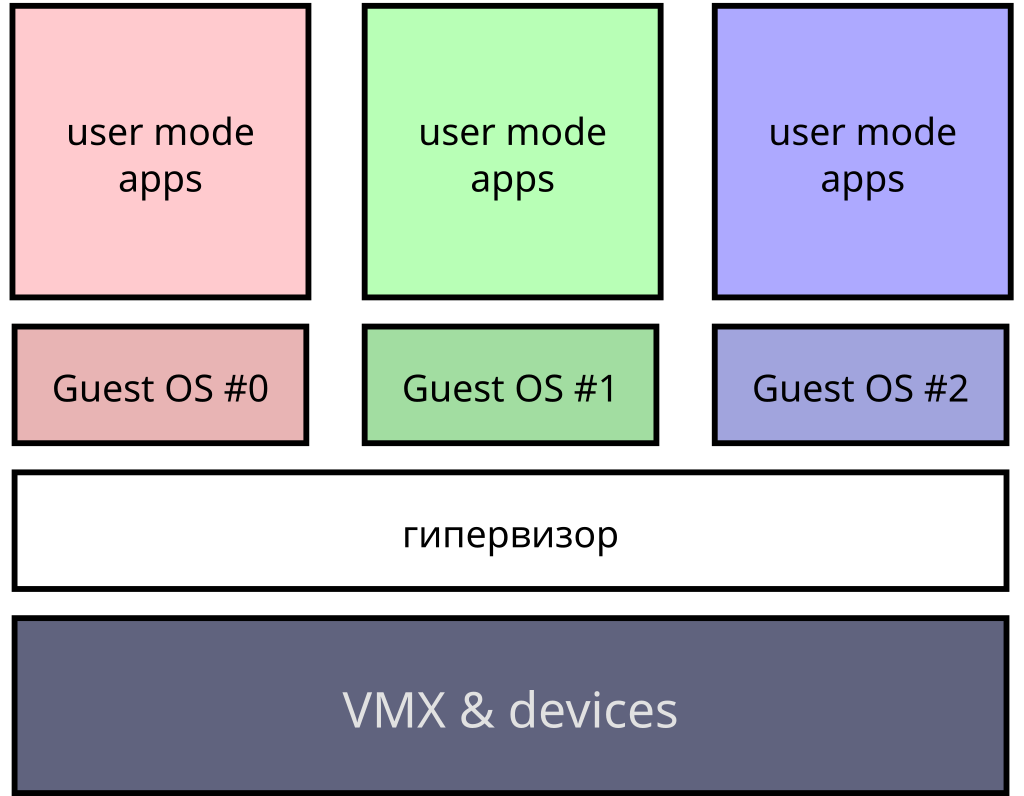
\includegraphics[width=0.9\textwidth]{../diagrams/hyper_type1} % first figure itself
				\caption{I тип гипервизоров}
				\label{fig:hypertype1}
			\end{minipage}\hfill
			\begin{minipage}{0.45\textwidth}
				\centering
				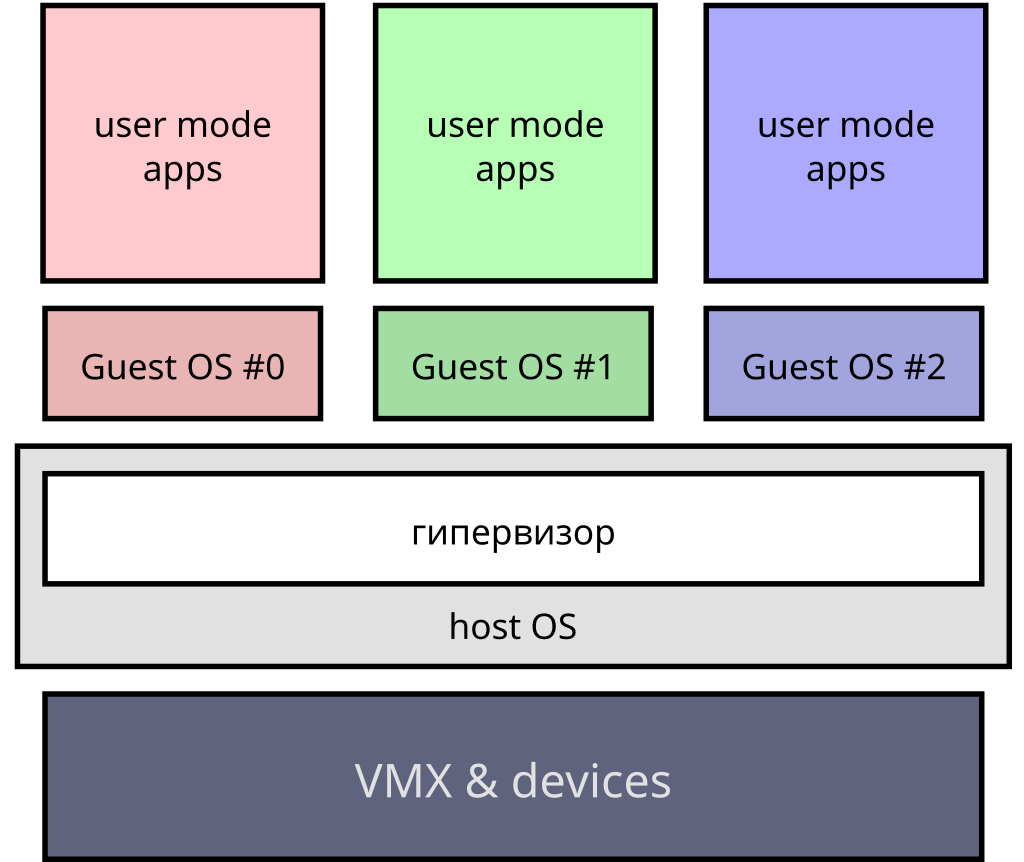
\includegraphics[width=0.9\textwidth]{../diagrams/hyper_type2}
				\caption{II тип гипервизоров}
				\label{fig:hypertype2}
			\end{minipage}
		\end{figure}
		Гипервизор Jinet - гипервизор I типа: так легче обращаться к ресурсам компьютера.
	\end{itemize}
	\section{Обзор аналогов}
	В данной работе представляется маленький гипервизор. Подобные ему большие аналоги писали десятки программистов много месяцев. Гипервизор Jinet сейчас позволяет запускать простейший код в изолируемом окружении ВМ виртуальной машины. У всех из предложенных ниже гипервизоров исходный текст находится в открытом доступе. Приведённые аналоги были написаны специалистами в области информационной безопасности и системного программирования. Некоторые из предложенных гипервизоров первого типа, а некоторые -- второго. \par
	\setlength{\extrarowheight}{20pt}
	\begin{table}[htb]
		\centering
		\caption{Аналоги}
		\vspace{0.5cm}
		\label{tbl:analogs}
		\renewcommand\tabularxcolumn[1]{m{#1}}% for vertical centering text in X column
		\begin{tabularx}{\textwidth}{|X|X|X|X|X|}
			\hline
			Гипервизор     & Тип VMM\footnotemark{} & Платформы\newline(если II тип)         & Размер\newline исходного текста & Назначение                  \\ \hline
			SimpleVisor    & II      & Win8.1; частично UEFI           & 162 KB                  & использование новейшего VMX \\ \hline
			Ramooflax      & I       & --                              & 2.26 MB                 & анализ/отладка\newline /контроль ВМ  \\ \hline
			HyperPlatform  & II      & Win7; Win8.1; Win10: x86 \& x64 & 7.64 MB                 & анализ\newline работы Windows       \\ \hline
			\textbf{Jinet} & I       & --                              & 421 KB                  & учебный\newline гипервизор \\ \hline
		\end{tabularx}
	\end{table}
	\footnotetext{см. \ref{sssec:hyptype}}
	\pagebreak
	\section{Программная реализация}
	Гипервизор Jinet был написан на языках программирования ассемблер (диалекты \texttt{fasm} и \texttt{as}) и C (компилятор \texttt{gcc}). Сборка проекта осуществляется с помощью сборщика \texttt{gnu ld} и утилиты \texttt{gnu make}. В качестве системы контроля версий используется \texttt{git} и хостинг GitHub.\par
	\section{Пример использования}
	\begin{figure}[htb]
		\centering
		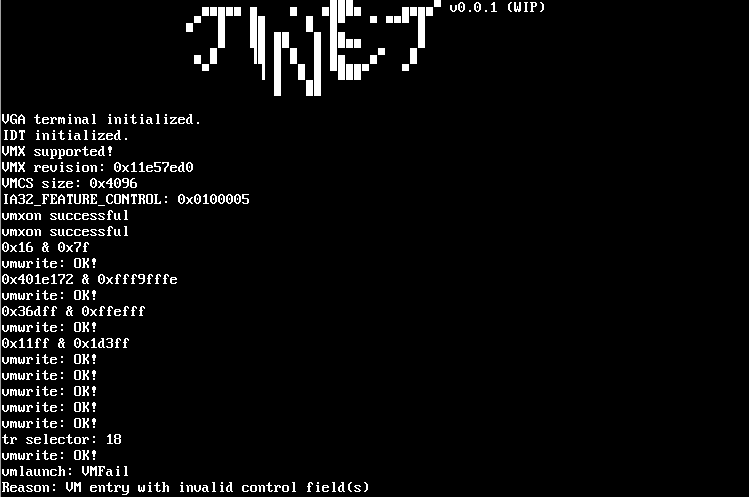
\includegraphics[width=0.55\linewidth]{../diagrams/jinet_vesa}
		\caption{Работа программы (VESA-режим)}
		\label{fig:jinetvesa}
	\end{figure}
	На \cref{fig:jinetvesa} изображена работа гипервизор Jinet. На данный момент гиперивизор поддерживает работу виртуальной машины, которая выводит сообщение о своём успешном запуске с помощью vmcall: \texttt{Hello! I am VM1!}.
	\section{Результат}
	\textbf{Была изучена архитектура процессоров Intel x86.} За время работы над гипервизором пришлось изучить самые разные аспекты работы современных ПК: от работы в 16-битном режим до опыта неуспешной отладки на разработческих платах.\par
	\textbf{Был получен важный опыт работы с технической документацией.} Большая часть документации, изученной во время работы над дипломным проектом, была написана на техническом английском. При работе с такой низкоуровневой технологией, как аппаратная виртуализация, была важно консультироваться со справочниками и документацией Intel.\par
	\textbf{Был изучен инструментарий современного системного программиста.} Основы статического компонования, формат исполняемых файлов \texttt{elf}, особенности встроенного ассемблера gcc -- самые разные технологии системного программирования были изучены при написании данной работы. Изучались также утилиты для сборки: были написаны скрипты для сборки проекта утилитами \texttt{gnu make} и \texttt{gnu ld}, а также Python-скрипт для конфигурирования проекта.\par
	\textbf{Были изучены основы работы с языком ассемблер и работы с большими проектами на C.} Были изучены три диалекта языка ассемблер: \texttt{masm}, \texttt{fasm} и \texttt{gnu as}. В работу вошёл код, написанный на последних двух. Также были изучены принципы написания интерфейсов и безопасного программирования на C.\par
	% \pagebreak
	\section{Выводы}
	\textbf{Создан гипервизор Jinet.} Доказано, что можно написать гипервизор силами одного человека в короткие сроки. Многое ещё требует реализации и улучшения:
	\begin{enumerate}
		\item Доработка SeaBIOS для поддержки запуска 16-битных операционных систем
		\item Поддержка ряда устройств для запуска одного из вариантов DOS
		\item Поддержка гипервизором работы на нескольких ядрах, процессорах
		\item Поддержка NUMA-систем
		\item Поддержка технологии Intel GVT-g (представлена в 2015), делающей возможной аппаратную виртуализацию видеоадаптеров для ВМ
	\end{enumerate}
	\section{Список литературы}
	\nocite{*}
	\renewcommand{\section}[2]{}%
	\bibliographystyle{../utf8gost705u}
	\bibliography{../biblio}
\end{document} % конец документа

